% Copyright (c) 2017 Victorien Elvinger
% Code licensed under GPLv3 (https://www.gnu.org/licenses/gpl-3.0.en.html).
% Content licensed under CC-BY 4.0 (https://creativecommons.org/licenses/by/4.0/).

\documentclass[xcolor=table]{beamer}
\usetheme{metropolis}

\usepackage[utf8]{inputenc}
\usepackage{amsmath}
\usepackage{hyperref}
\hypersetup{colorlinks=true,urlcolor=blue}

% meta-data
% ---------

\author{Victorien Elvinger}
\title{\$ SHELL}
\institute{
\includegraphics[scale=0.2]{fig/ul-logo.pdf}\hspace{0.3em}Université de Lorraine - Telecom Nancy}
\date{Octobre 2017}

% Presentation
% ------------

\begin{document}

\maketitle

\begin{frame}{Commandes}
\begin{itemize}
    \item Chaque paramètre est séparé par un espace
    \begin{figure}
    
\includegraphics[scale=0.5]{fig/command.pdf}
    \end{figure}
    \item Ex. \textbf{-l} et \textbf{$\backsim$/Desktop} sont deux paramètres passés à \textbf{ls}
    \begin{figure}
    
\includegraphics[scale=0.5]{fig/command-example.pdf}
    \end{figure}
    \item Les guillemets simples permettent de passer des paramètres qui incluent des espaces ou des caractères spéciaux (\$, *, ...)
    \begin{figure}
    
\includegraphics[scale=0.5]{fig/command-example-with-single-quotes.pdf}
    \end{figure}
\end{itemize}
\end{frame}

\begin{frame}{Motifs de fichiers}
\begin{itemize}
    \item Désigne un ensemble de fichiers\\
    ex. tous les fichiers avec l'extension $.jpg$
    \item Composé de caractères spéciaux
    \begin{itemize}
        \item \textbf{?} représente n'importe quel caractère
        \item \textbf{*} représente n'importe quel nombre (incluant aucun) de un ou plusieurs caractère-s
        \item ... voir Wikipedia (\href{https://en.wikipedia.org/wiki/Glob_(programming)}{glob programming})
    \end{itemize}
    ex. \textbf{*.jpg}
\end{itemize}
\end{frame}

\begin{frame}{Résolutions de motifs de fichiers}
\begin{itemize}
    \item Le shell résout les motifs de fichiers avant l'exécution de la commande
    \begin{figure}
    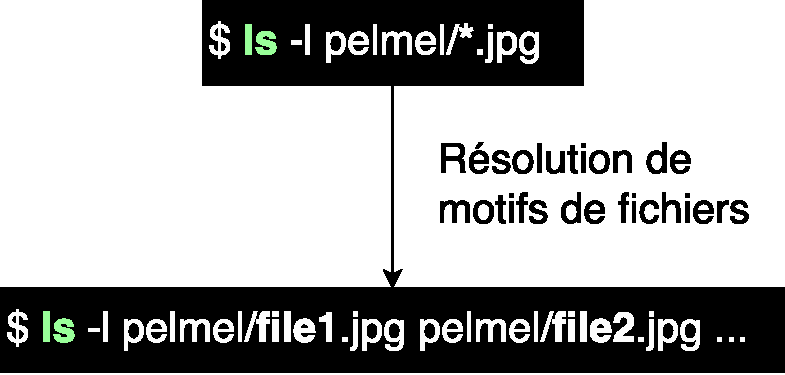
\includegraphics[scale=0.5]{fig/file-pattern.pdf}
    \end{figure}
\end{itemize}
\end{frame}

\begin{frame}{Exercies : Motifs de fichiers}
\begin{itemize}
    \item Quel motif désigne les fichiers dont le nom débute par \textbf{td} ?
    \item Quel motif désigne les photos d'extension \textbf{jpg} dont le nom contient \textbf{2017} ?
    \item Quel motif désigne les ficheirs qui contiennent au moins un espace ?
\end{itemize}
\end{frame}

\begin{frame}{Correction : Motifs de fichiers}
\begin{itemize}
    \item Quel motif désigne les fichiers dont le nom débute par \textbf{td} ?
    \begin{itemize}
        \item \textbf{td*}
    \end{itemize}
    \item Quel motif désigne les photos d'extension \textbf{jpg} dont le nom contient \textbf{2017} ?
    \begin{itemize}
        \item \textbf{2017*.jpg}
    \end{itemize}
    \item Quel motif désigne les ficheirs qui contiennent au moins un espace ?
    \begin{itemize}
        \item \textbf{*' '*}
    \end{itemize}
\end{itemize}
\end{frame}

\begin{frame}{Entrée / Sortie Standards}
\begin{itemize}
    \item Un programme peut
    \begin{itemize}
        \item recevoir des données sur l'Entrée Standard
        \item rendre des résultats sur la Sortie Standard
    \end{itemize}
    \item Ne pas confondre paramètres et entrée standard
    \begin{figure}
    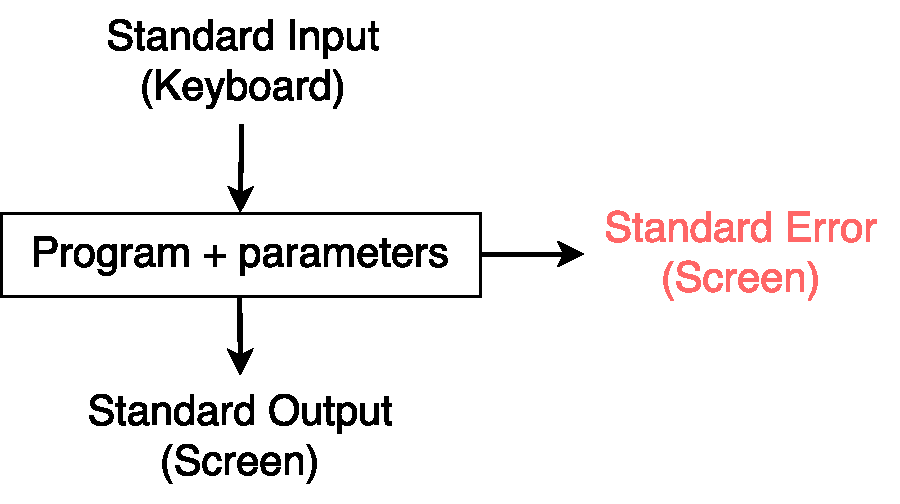
\includegraphics[scale=0.5]{fig/in-out.pdf}
    \end{figure}
\end{itemize}
\end{frame}

\begin{frame}{Entrée / Sortie Standards - Exemple}
\begin{enumerate}
    \item Le programme \textbf{cowsay -f duck} est lancé
    \item L'utilisateur imprime "hello" sur l'entrée standard et valide
    \item Le programme imprime le résultat sur la sortie standard
\end{enumerate}
\begin{figure}
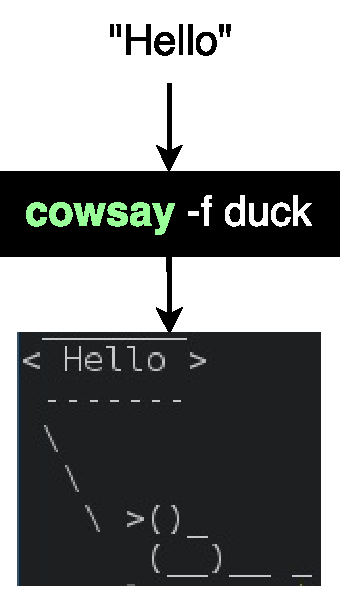
\includegraphics[scale=0.5]{fig/in-out-example.pdf}
\end{figure}
\end{frame}

\begin{frame}{Redirections des E/S}
\begin{itemize}
    \item $command > file.txt$ \\$command >> file.txt$
    \begin{itemize}
        \item Redirige la sortie standard vers un fichier
        \item $>$ écrase le fichier si il existe
        \item $>>$ ajoute le contenu à la fin du fichier
    \end{itemize}
    \item $command < file.txt$
    \begin{itemize}
        \item Utilise un fichier comme entrée standard
    \end{itemize}
    \item $command1 \,|\, command2$
    \begin{itemize}
        \item Redirige la sortie standard d'un premier programme vers l'entrée standard d'un second programme
    \end{itemize}
\end{itemize}
\end{frame}

\begin{frame}{Exemples de redirections}
\begin{itemize}
    \item \textbf{cowsay -f duck $<$ file.text} utilise le contenu de file.text comme message
    \item \textbf{echo Hello $|$ cowsay -f duck $|$ cowsay -n -f duck}
    \begin{figure}
        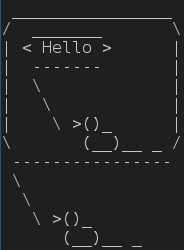
\includegraphics[scale=0.4]{fig/cowsay-inception.png}
    \end{figure}
    \item \textbf{yes $|$ apt install} permet d'imprimer "y" (yes) à chaque fois que le programme attend une entrée
\end{itemize}
\end{frame}

\begin{frame}{Variables}
\begin{itemize}
    \item Préfixées par \textbf{\$}
    \begin{itemize}
        \item \textbf{\$HOME} contient le chemin absolu du dossier personnel de l'utilisateur courrant
        \item \textbf{\$PATH} contient les chemins absolus vers les dossiers dans lesquels les programmes sont recherchés
    \end{itemize}
    \item \textbf{a=1} déclare ou modifie la variable \textbf{\$a} avec la valeur \textbf{1}\\
    Pas d'espace autour de \textbf{=}
    \item \textbf{unset a} supprime la variable \textbf{\$a}
\end{itemize}
\end{frame}

\begin{frame}{Substitutions de variables}
\begin{itemize}
    \item Le Shell remplace les variables par leur valeurs avant d'exécuter la commande
    \begin{figure}
        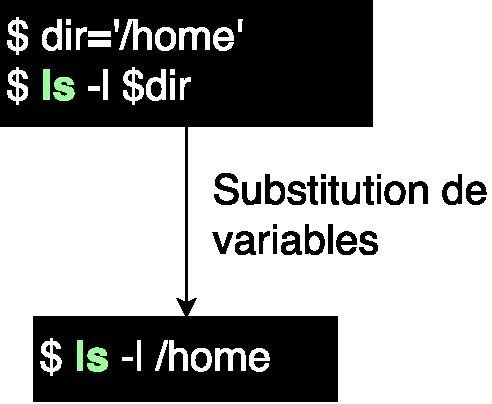
\includegraphics[scale=0.5]{fig/var-substitution.pdf}
    \end{figure}
\end{itemize}
\end{frame}

\begin{frame}{Substitutions de variables et paramètres}
\begin{itemize}
    \item La valeur d'une variable peut contenir des espaces
    \begin{itemize}
        \item Une substitution peut donc produire plusieurs paramètres
        \item Les guillemets double permettent de substituer une variable en un seul paramètre
    \end{itemize}
    \item Une variable devrait toujours être entourée de guillemets double (à quelques rares exceptions)
    \begin{figure}
        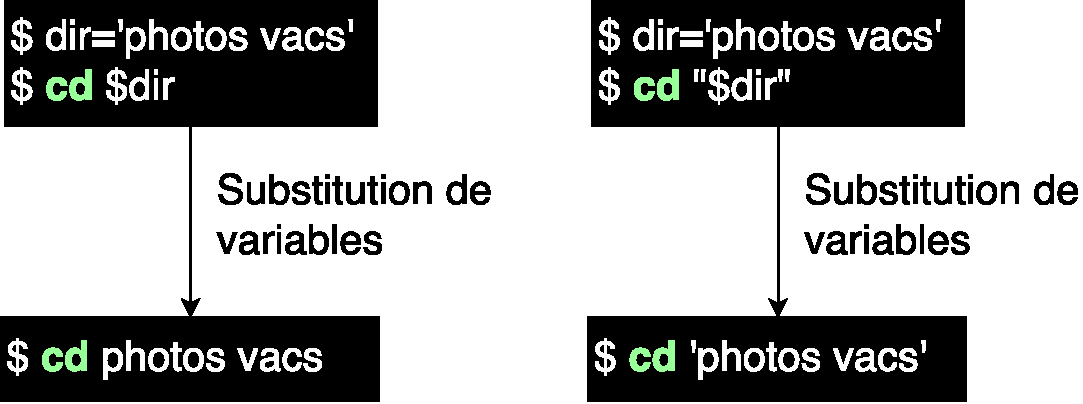
\includegraphics[scale=0.5]{fig/double-quoted-var.pdf}
    \end{figure}
\end{itemize}
\end{frame}

\begin{frame}{Fichiers / Scripts exécutables}
\begin{itemize}
    \item Est autorisé à être exécuté
    \begin{itemize}
        \item \textbf{chmod u+x script}
    \end{itemize}
    \item Ecrit pour un interpréteur (python, node, sh, bash, ...)
    \item Un shebang \textbf{\#!} indique au Shell quel interpréteur utiliser
    \begin{itemize}
        \item Placé sur la première ligne du fichier
        \item Suivi par le chemin absolu de l'interpréteur\\
        \textbf{\#!~/bin/sh}\\
        \textbf{\#!~/bin/bash}\\
        \textbf{\#!~/usr/bin/python}
    \end{itemize}
    \item Si l'interpréteur n'est pas indiqué, le Shell essaye de l'interpréter
\end{itemize}
\end{frame}

\begin{frame}{POSIX}
\begin{itemize}
    \item POSIX offre un standard pour le langage Shell
    \begin{itemize}
        \item Voir \href{http://pubs.opengroup.org/onlinepubs/009695399/utilities/xcu_chap02.html}{Shell Command Language}
    \end{itemize}
    \item Bash respecte en grande partie POSIX et offre beaucoup de structures supplémentaires
    \begin{itemize}
        \item Si vous avez un doute, préférez toujours utiliser \textbf{\#!~/bin/bash} au lieu de \textbf{\#!~/bin/sh}
    \end{itemize}
    \item Dans ce cours nous apprenons les bases de POSIX
    \begin{itemize}
        \item Nous utiliserons donc \textbf{\#! /bin/sh}
    \end{itemize}
\end{itemize}
\end{frame}

\begin{frame}{Exercice : separer}
\begin{itemize}
    \item Ecrire un script nommé \textbf{separer} qui déplace les fichiers d'extension \textbf{jpg} du sous-dossier \textbf{pelmel} vers un sous-dossier \textbf{sep}
    \item Que pourrions-nous faire pour le rendre plus générique ?
\end{itemize}
\end{frame}

\begin{frame}{Correction : separer}
\#!/bin/sh\\
mkdir sep\\
mv pelmel/*.jpg sep/
\end{frame}

\begin{frame}{Récupération de paramètres}
\begin{itemize}
    \item \textbf{\$0} est le nom du script / programme tel que appelé
    \item \textbf{\$n} est le n-éme paramètre
    \item \textbf{\$\#} est le nombre de paramètres
    \item \textbf{\$*}, \textbf{\$@} est la liste des paramétres séparés par des espaces
\end{itemize}
\end{frame}

\begin{frame}{Exercice : separer avec paramétres}
\begin{itemize}
    \item Adapter le script \textbf{separer} pour qu'il déplace les fichiers d'une extension particulière d'un dossier donné vers un sous-dossier \textbf{sep}
    \begin{itemize}
        \item ./separer jpg pelmel
        \item ./separer txt pelmel
    \end{itemize}
    \item Que pourrions-nous faire pour le rendre plus robuste ?
\end{itemize}
\end{frame}

\begin{frame}{Correction : separer avec paramétres}
\#!/bin/sh\\
mkdir sep\\
mv "\$2"/*."\$1" sep/
\end{frame}

\begin{frame}{Exit Status}
\begin{itemize}
    \item L'exécution d'une commande réussit ou échoue
    \item Après son exécution, une commande renvoie un statut qui est un entier naturel
    \begin{itemize}
        \item \textbf{0} indique un succès
        \item Un entier plus grand que 0 indique un échec
    \end{itemize}
    \item \textbf{exit n} retourne le statut $n$ au Shell appelant
\end{itemize}
\end{frame}

\begin{frame}{Programme test ou [}
\begin{itemize}
    \item \textbf{test EXPR} ou \textbf{[ EXPR ]} permet de tester des conditions
    \begin{itemize}
        \item \textbf{[ 'abc e' = 'abc e' ]} \quad exit status: 0
        \item \textbf{[ "\$var" != 'a' ]} \quad pour var=a, exit status: 1
        \item \textbf{[ 1 -eq 1 ]} \quad exit status: 0
        \item \textbf{[ 1 -lt 2 -a 2 -gt 1 ]} \quad exit status: 0
    \end{itemize}
    \item \textbf{]} est un paramètre obligatoire de la commande \textbf{[}
    \item Ne pas oublier les espaces entre chaque paramètres
    \item Voir le manuel d'utilisation (\textbf{man test} ou \textbf{man [})
\end{itemize}
\end{frame}

\begin{frame}{Instruction conditionnelle}
\textbf{if} command\\
\textbf{then}\\
\quad \# command has 0 as exit status\\
\quad command1\\
\textbf{else}\\
\quad command2\\
\textbf{fi}\\
\end{frame}

\begin{frame}{Itérations : tant-que}
\textbf{while} command\\
\textbf{do}\\
\quad \# command has still 0 as exit status\\
\quad command1\\
\textbf{done}\\
\end{frame}

\begin{frame}{Exercice : choix}
\begin{itemize}
    \item Écrire un programme qui boucle sur l'entrée standard jusqu'à obtenir la chaîne de caractères "yes" ou "no" et l'imprimer sur la sortie standard
    \item \textbf{read answer} lit une ligne sur l'entrée standard et l'écrit dans la variable \textbf{\$answer}
    \item Une amélioration possible est de personnaliser le choix
    \begin{itemize}
        \item \textbf{choix a b} attend \textbf{a} ou \textbf{b}
    \end{itemize}
\end{itemize}
\end{frame}

\begin{frame}{Instruction d'itérations : for-in}
\textbf{for} var \textbf{in} sequence\\
\textbf{do}\\
\quad command1\\
\textbf{done}\\
unset var\\
\begin{itemize}
    \item La séquence est un ensemble de valeurs séparées par des espaces
    \begin{itemize}
        \item \textbf{1 2 3}
        \item \textbf{alice karim tristan hadjer}
        \item \textbf{'first element' 'second element'}
    \end{itemize}
\end{itemize}
\end{frame}

\begin{frame}{Séquence "\$@"}
\begin{itemize}
    \item \textbf{"\$@"} a une régle de substitution particulière
    \begin{itemize}
        \item \textbf{"\$@"} est équivalent à \textbf{"\$1" "\$2" ...}
        \item \textbf{"\$@"} est donc la séquence des paramètres
    \end{itemize}
    \item A l'inverse \textbf{"\$*"} suit la régle de substitution usuelle
    \begin{itemize}
        \item \textbf{"\$*"} est équivalent à \textbf{"\$1 \$2 ..."}
        \item \textbf{"\$*"} est donc une séquence avec un seul élément
    \end{itemize}
\end{itemize}
\end{frame}

\begin{frame}{Exercice : enlever}
\begin{itemize}
    \item Écrire un programme qui enlève un nom d'une séquence de noms
    \begin{itemize}
        \item \textbf{enlever tristan alice karim tristan hadjer}\\
        imprime sur la sortie standard :\\
        \textbf{alice karim hadjer}
    \end{itemize}
    \item \textbf{shift} décale les paramètres\\
    \$j devient \$i avec j = i + 1\\
    Attention : \$0 est inchangé\\
    \$\# est décrémenté de un
    \item L'option \textbf{-n} de \textbf{echo} empêche \textbf{echo} d'imprimer un retour à la ligne
\end{itemize}
\end{frame}

\begin{frame}{Substitution de commandes}
\begin{itemize}
    \item \textbf{\$(command)} est substitué par ce qui est imprimé sur la sortie standard par \textbf{command}
    \item \textbf{\`\,command\`} (backquotes) est l'ancienne syntaxe de \textbf{\$(command)}
    \item Exemples
    \begin{itemize}
        \item cowsay -f "\$(choix duck tux)" $<$ file.txt
        \item enlever a \$(enlever b x y a c b)
    \end{itemize}
\end{itemize}
\end{frame}

\begin{frame}{Licence du contenu}
\href{https://creativecommons.org/licenses/by/4.0/}{CC-BY 4.0 - Attribution 4.0 International}
\end{frame}

\end{document}
